\documentclass{amsart}
\usepackage[utf8]{inputenc}
\usepackage{accents}
\usepackage{graphicx}
\usepackage{amsfonts}
\usepackage{listings}
\usepackage{amscd}
\usepackage{amssymb}
\usepackage{hyperref}
\usepackage{url}
\usepackage{tikz}
\usepackage[a4paper,margin=1in]{geometry}
\newtheorem{theorem}{Theorem}
\newtheorem{lemma}[theorem]{Lemma}
\newtheorem{corollary}[theorem]{Corollary}
\newtheorem{proposition}[theorem]{Proposition}
\theoremstyle{definition}
\newtheorem{definition}[theorem]{Definition}
\newtheorem{example}[theorem]{Example}
\theoremstyle{remark}
\newtheorem{remark}[theorem]{Remark}
\newcommand{\abs}[1]{\lvert#1\rvert}
\newcommand{\ZZ}{\mathbb Z}
\newcommand{\QQ}{\mathbb Q}
\newcommand{\RR}{\mathbb R}
\newcommand{\NN}{\mathbb N}
\newcommand{\CC}{\mathbb C}
\newcommand{\From}{\colon}
\newcommand{\To}{\rightarrow}

\lstset{
language=R,
basicstyle=\scriptsize\ttfamily,
commentstyle=\ttfamily\color{gray},
numbers=left,
numberstyle=\ttfamily\color{gray}\footnotesize,
stepnumber=1,
numbersep=5pt,
backgroundcolor=\color{white},
showspaces=false,
showstringspaces=false,
showtabs=false,
frame=single,
tabsize=2,
captionpos=b,
breaklines=true,
breakatwhitespace=false,
title=\lstname,
escapeinside={},
keywordstyle={},
morekeywords={},
numbers=none
}


%---------EDIT THE CONTENTS TITLE/AUTHOR INFO BELOW!
\title{YSC4204: Statistical Computing\\
Problem Set 2}
\author{East: Sean Saito, John Reid, Hrishi Olickel, Chong Woon Han}
\date{\today}

%-----------THIS IS WHERE THE GOOD STUFF BEGINS.
\begin{document}

\maketitle

\begin{enumerate}
%1
\item
The C code to implement meanC() is as follows:
\begin{lstlisting}[language=C]
#include <stdio.h>
#include <R.h>

/*
* Function that calculates the mean of vector x
* Inputs:
*     x   : vector of doubles
*     n   : length of vector
*     res : placeholder for result
*/
void meanC(double *x, int *n, double *res) {

  int i;
  double temp = 0.0;
  for (i = 0; i < *n; i++) {
    temp += x[i];
  }

  *res = temp / *n;
  return;
}
\end{lstlisting}
We call this function in R using the following R Code:
\begin{lstlisting}[language=R]
# Automatically sets working directory to source file location
this.dir <- dirname(parent.frame(2)$ofile)
setwd(this.dir)

# Problem 1 - Writing a mean function in C to be used in R
meanR <- function(x) {
  # Placeholder for result
  res = 0.0
  n = length(x)
  
  dyn.load("mean.so")
  m = .C("meanC", x=as.double(x), n=n, res=res)
  
  return(m$res)
}
\end{lstlisting}
%2
\item
\begin{enumerate}
%a
\item
With reference to Figure 2, let the red line (the "radius") be $y_1$ and let the blue line (the chord) be $y_2$. 

We need to find the point $(p_1,q_1)$. To do so, we will first find the lines $y_1$ and $y_2$, then "step" from $(p_0,q_0)$ to $(p_1,q_1)$ by adding the distance from $(p_0,q_0)$ to the midpoint.
\begin{align*}
y_1 &= \frac{q}{2p}x. \hspace{0.5cm} \text{(Since } y_1 \text{ bisects the perpendicular from } (p_0,q_0) \text{ to the } x \text{-axis)}\\
y_2 &= \frac{-2p}{q}x + c. \hspace{0.5cm} \text{Substitute in } (p,q)\\
q &= \frac{-2p}{q} \cdot p + c.\\
q^2 &= -2p^2 + qc.\\
c &= \frac{q^2+2p^2}{q}.\\
\Rightarrow y_2 &= \frac{-2p}{q}x + \frac{q^2 + 2p^2}{q}.
\end{align*}
We need to find the intersection of $y_1$ and $y_2$, so we set $y_1 = y_2$.
\begin{align*}
\frac{qx}{2p} &= \frac{-2px}{q} + \frac{q^2+2p^2}{q},\\
q^2x+4p^2x &= 2pq^2 +4p^3,\\
x(q^2+4p^2) &= 2pq^2+4p^3,\\
x &= \frac{2pq^2 +4p^3}{q^2+4p^2}.
\end{align*}
To find $y$, we substitute $x$ into the equation for $y_1$,
\begin{align*}
y &= \frac{q}{2px},\\
&= \frac{q}{2p} \cdot \bigg( \frac{2pq^2 + 4p^3}{q^2+4p^2} \bigg),\\
&= \frac{2pq^3+4p^3q}{2pq^2+8p^3},\\
&= \frac{q^3+2p^2q}{q^2+4p^2}.
\end{align*}
Now we need to find $(p_1,q_1)$. We know that the distance from $(p_0,q_0)$ to the midpoint is equal to the distance from the midpoint to $(p_1,q_1)$. Breaking it into components:
\begin{align*}
p_1 &= p_0 + 2(p_2-p_0), \hspace{0.5cm} \text{where } p_2 \text{ is the } x \text{-coordinate of the mid point}\\
&= 2p_2 - p_0.
\end{align*}
Similarly, $q_1 = 2q_2 - q_0$.
\begin{align*}
p_1 &= 2p_2-p,\\
&= 2 \bigg( \frac{2pq^2 + 4p^3}{q^2+4p^2} \bigg) - p,\\
&= \frac{4pq^2 + 8p^3 - pq^2 - 4p^2}{q^2+4p^2},\\
&= \frac{3pq^2 + 4p^3}{q^2+4p^2},\\
&= \frac{p(4p^2 + q^2) + 2pq^2}{4p^2+q^2},\\
&= p + 2p \bigg( \frac{q^2}{4p^2+q^2} \bigg),\\
&= p ( 1+2 \bigg( \frac{\frac{q^2}{p^2}}{4 + \frac{q^2}{p^2}} \bigg) ),\\
&= p (1 + 2 \bigg( \frac{r}{4+r} \bigg),\\
&= p (1 + 2s).
\end{align*}
\begin{align*}
q_1&= 2q_2 - q_0,\\
&= 2 \bigg( \frac{q^3 + 2p^2q}{q^2+4p^2} \bigg) - q,\\
&= \frac{2q^3+4p^2q - q^3 - 4p^2q}{q^2+4p^2},\\
&= \frac{q^3}{q^2+4p^2},\\
&= q \cdot \frac{q^2}{q^2+4p^2},\\
&= q \cdot \bigg( \frac{q^2}{p^2} \cdot \frac{p^2}{4p^2+q^2} \bigg),\\
&= q \cdot \Bigg( \frac{r}{\frac{4p^2+q^2}{p^2}} \Bigg),\\
&= q \cdot \bigg( \frac{r}{4+r} \bigg) ,\\
&= q \cdot s .
\end{align*}

We've just shown that $(p_1, q_1)$ are the same as the values of $p$ and $q$ after the $k=1$ iteration of the loop. Since both points lie on the circle, $\sqrt{p_1^2+q_1^2} = \sqrt{a^2+b^2}$. Hence we can consider this to be the loop invariant. For each iteration, the line from $(0,0)$ to $(p_k, q_k)$ remains on the circle while moving towards the x axis. This means $$\lim_{k\to\infty}q_k = 0 \Rightarrow \lim_{k\to\infty}p_k = \sqrt{a^2+b^2}.$$ This becomes true when $q_k$ becomes insignificant. In practice however, 3 iterations are necessary to approach decent accuracy, hence the limit of $k=3$.
\\
%b
\item 

There are two cases where \textbf{pythag2} fails and \textbf{pythag} works:

\begin{lstlisting}[language=R]
x = 3e200
y = 4e200
pythag2(x,y)
> [1] Inf
pythag(x,y)
> [1] 5e200
x = 3e-200
y = 4e-200
> pythag2(x,y)
[1] 0
> pythag(x,y)
[1] 5e-200
\end{lstlisting}

The reason \textbf{pythag2} fails while \textbf{pythag} runs is due to possible overflow and underflow generated in the intermediate result of $x^2+y^2$. For extremely large and small numbers, this value will limit the possible inputs of $x$ and $y$ to a range smaller than that of allowed by the floating points being used. \textbf{pythag} prevents this by iteratively approximating the value, where $p$ approaches the result. 
\\
\end{enumerate}
%3
\item
The standard Laplacian distribution is given by $f(x)  = \frac{1}{2} e ^{|x|}$. 
\newline
To obtain the inverse transform $F^{-1}_X(x)$, we must first take the integral of $f(x)$, and then find the inverse of the integral. 

We will first separate $f(x)$ into cases
$$f_X(x) = \begin{cases}
    \frac{1}{2}e^{x} & \text{     if $x < 0$} \\
    \frac{1}{2}e^{-x} & \text{if $x >= 0$}
    \end{cases}
$$

Taking the integral, we get

$$F_X(x) = \begin{cases}
    \frac{1}{2}e^{x} & \text{if $x < 0$} \\
    1 - \frac{1}{2}e^{-x} & \text{if $x >= 0$}
    \end{cases}
$$

For the second case, the indefinite integral gives us $- \frac{1}{2}e^{-x} + c$, and we need $F_X(x)$ to be a cumulative distribution, so we have $c = 1$. 

For the inverse transform, we must again do case analysis. For $F_X(x) = \frac{1}{2}e^{x}$: 

\begin{align*}
y &= \frac{1}{2}e^{x}\\
2y &= e^{x}\\
x &= \ln (2y).
\end{align*}

At $x = 0$, $F_X(x) = 0.5$, so this first case of the integral holds true for $x < 0.5$. 

Case 2: 
\begin{align*}
y &= 1 - \frac{1}{2}e^{-x}\\
y - 1 &= - \frac{1}{2} e^{-x}\\
2 - 2y &= e^{-x}\\
\ln{(2-2y)} &= -x\\
x &= -ln{(2-2y)}.
\end{align*}

This holds true for $x >= 0.5$.

Therefore, $F^{-1}_X(x)$ is given by the following
$$G_X(x) = \begin{cases}
    \ln{(2y)} & \text{if $x < 0.5$} \\
    \ln{(2 - 2y)} & \text{if $x >= 0.5$}
    \end{cases}
$$

This is easy to translate into R. 

\begin{lstlisting}[language=R]
# Define the standard laplacian pdf
laplacian_pdf <- function (x){
  return(0.5 * exp(-abs(x)))
}

# Define the laplacian cdf (not used)
laplacian_cdf <- function (x){
  return(ifelse(x < 0, 0.5*exp(x), 1 - 0.5*exp(-x)))
}

# Define the inverse transform of the laplacian cdf
inv_trf <- function (x){
  return(ifelse(x < 0.5, log(2*x), -log(2 - 2*x)))
}

# Generate the random sample
result <- inv_trf(runif(10000))

# Graph the sample
hist(result, probability = TRUE, breaks = 100,
     xlim = c(-5, 5), ylim = c(0,0.5))

# Overlay the line
x <- seq(-5,5,0.1)
y <- laplacian_pdf(x)
lines(x,y,col = "red")
\end{lstlisting}

The resulting histogram is shown below:\\
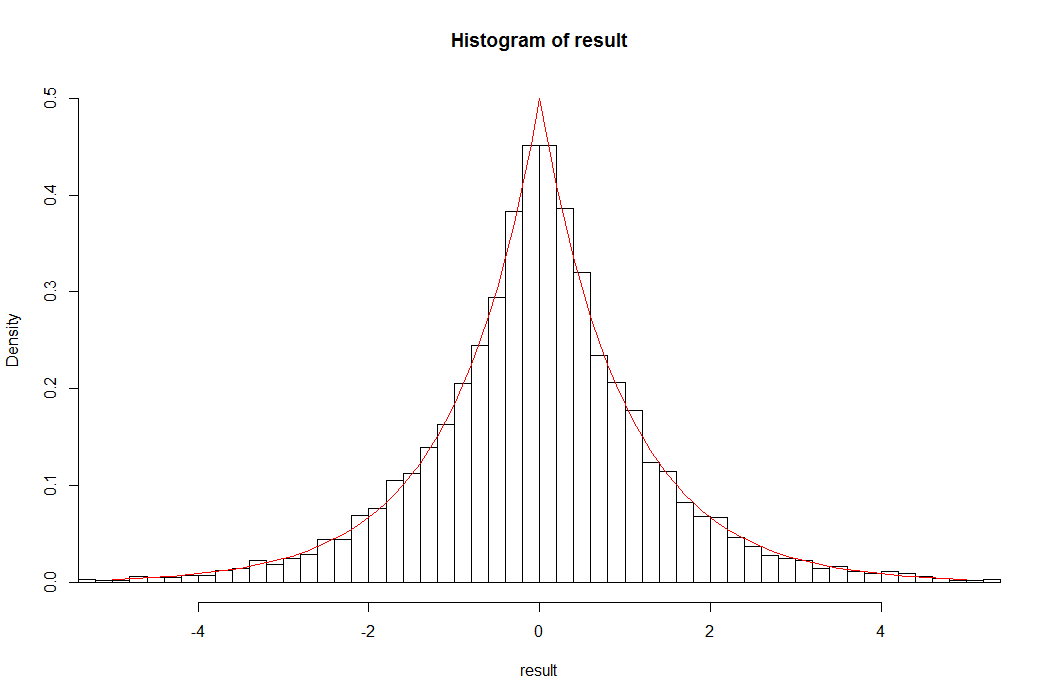
\includegraphics[scale=0.5]{laplacian}

%4
\item
Suppose $x \sim$ Rayleigh($\sigma$). The Rayleigh probability density function is
$$ f(x) = \frac{x}{\sigma^2}e^{-x^2/(2\sigma^2)}, \hspace{0.5cm} x \geq 0, \sigma >0.$$
The cumulative distribution function is
\begin{align*}
F_X(x) = \int \frac{x}{\sigma^2}e^{-x^2/(2\sigma^2)} dx,\\
\end{align*}
Let $u = -x^2/(2\sigma^2)$,
\begin{align*}
\frac{du}{dx} &= \frac{-x}{\sigma^2},\\
du &= \frac{-x}{\sigma^2}dx.
\end{align*}
By substitution,
\begin{align*}
F_X(x) &= \int -e^u du,\\
&= -e^u + c,\\
&= -e^{-x^2/(2\sigma^2)} + c.
\end{align*}
Observe that when $x=1, F_X(x)=0$. Therefore $c=1$. Thus, we have the cumulative distribution for the Rayleigh distribution,
$$ F_X(x) = 1 - e^{-x^2/(2\sigma^2)} \hspace{0.5cm} \text{ for } x \in [0,\infty).$$
We derive $F^{-1}_X(x)$ as follows:
\begin{align*}
y &= 1 - e^{-x^2/(2\sigma^2)},\\
e^{-x^2/(2\sigma^2)} &= 1-y,\\
\frac{-x^2}{2\sigma^2} &= \ln (1-y),\\
x &= \sqrt{-2\sigma^2 \ln (1-y)},\\
F^{-1}_X(x) &= \sqrt{-2\sigma^2 \ln (1-y)}.
\end{align*}
For $u \sim$ Uniform$(0,1)$, and given that $U$ and $1-U$ have the same distribution, we can generate Rayleigh random variables by taking
$$ F^{-1}_X(u) = \sqrt{-2\sigma^2 \ln (u)}.$$
We implement this equation in R to generate $n$ random samples from a Rayleigh($\sigma$) distribution as shown below:
\begin{lstlisting}[language=R]
## Define function to generate Rayleigh random variables ##
rray <- function(n,sigma){
  u <- runif(n)
  output <- sqrt(-2*sigma^2*log(u))
  return(output)
}
\end{lstlisting}
The code used to generate histograms is as follows:
\begin{lstlisting}[language=R]
## Set seed to ensure consistency before generating numbers and plotting ##
set.seed(0)

########## simga = 0.5 ##########
x1 <- rray(10000,0.5)
hist(x1,prob=TRUE,
 main="Generated rayleigh random variables with sigma=0.5",
 xlab="x") # plot the histogram

## Superimpose a density line ##
xlines1 <- seq(0,round(max(x1)),0.01)
ylines1 <- (xlines1/0.5^2)*exp(-xlines1^2/(2*(0.5^2)))
lines(xlines1,ylines1)

########## sigma = 2 ##########
x2 <- rray(10000,2)
hist(x2,prob=TRUE,
 main="Generated rayleigh random variables with sigma=2",
 xlab="x") # plot the histogram

## Superimpose a density line ##
xlines2 <- seq(0,round(max(x2)),0.01)
ylines2 <- (xlines2/2^2)*exp(-xlines2^2/(2*(2^2)))
lines(xlines2,ylines2)
\end{lstlisting}
The resulting histograms are show below:\\
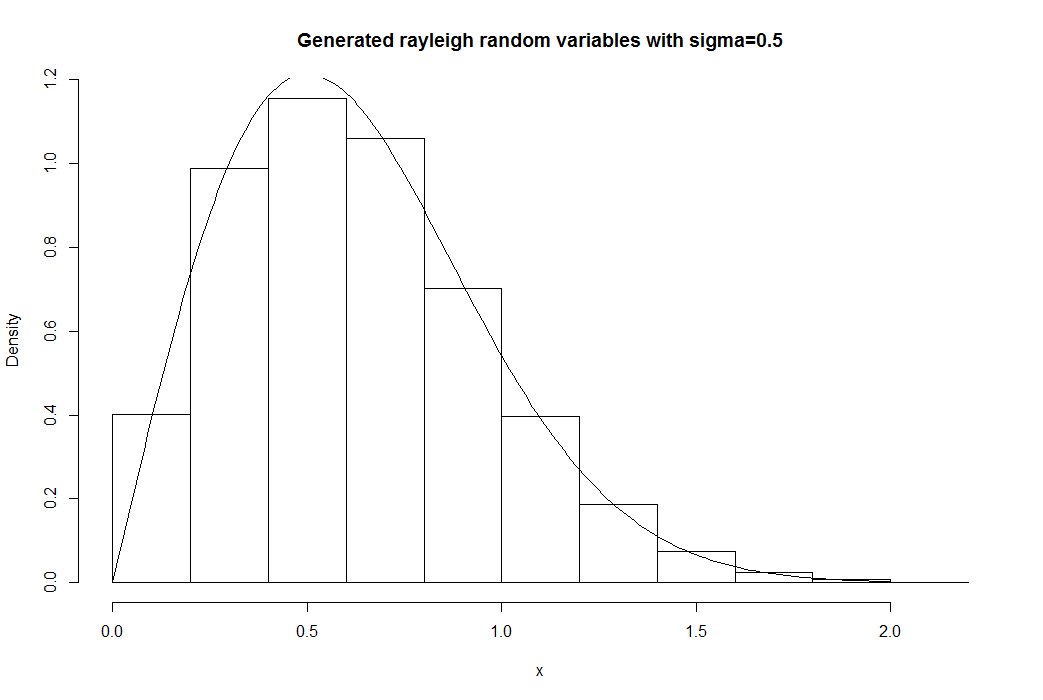
\includegraphics[scale=0.6]{rayleigh_0_5}
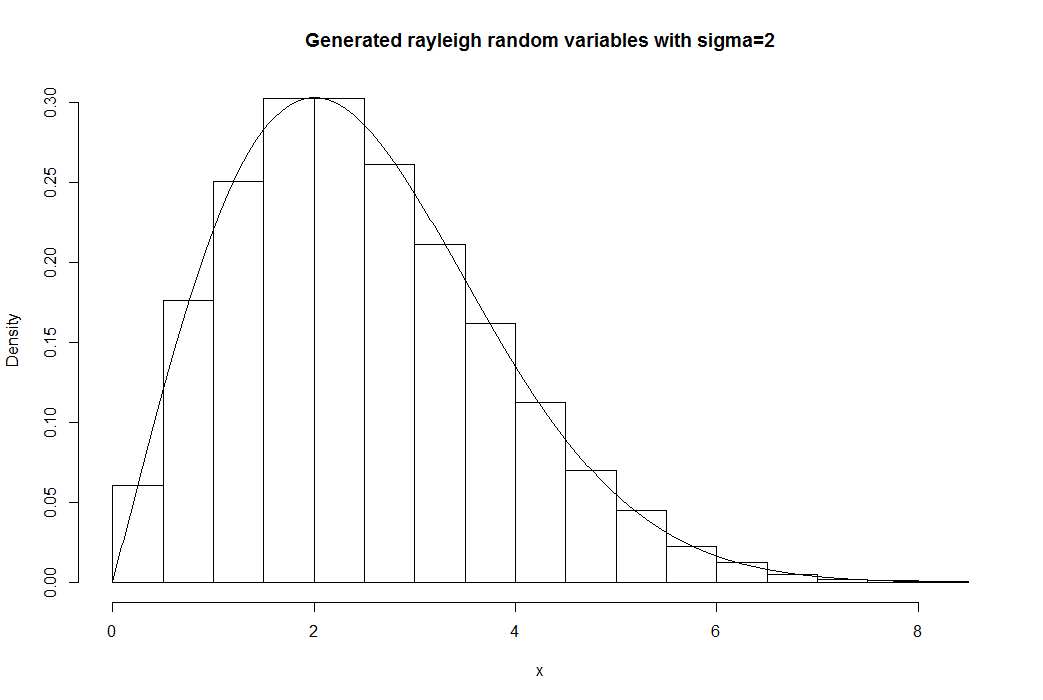
\includegraphics[scale=0.6]{rayleigh_2}
\end{enumerate}
\end{document}
